% Options for packages loaded elsewhere
\PassOptionsToPackage{unicode}{hyperref}
\PassOptionsToPackage{hyphens}{url}
%
\documentclass[
]{article}
\usepackage{amsmath,amssymb}
\usepackage{iftex}
\ifPDFTeX
  \usepackage[T1]{fontenc}
  \usepackage[utf8]{inputenc}
  \usepackage{textcomp} % provide euro and other symbols
\else % if luatex or xetex
  \usepackage{unicode-math} % this also loads fontspec
  \defaultfontfeatures{Scale=MatchLowercase}
  \defaultfontfeatures[\rmfamily]{Ligatures=TeX,Scale=1}
\fi
\usepackage{lmodern}
\ifPDFTeX\else
  % xetex/luatex font selection
\fi
% Use upquote if available, for straight quotes in verbatim environments
\IfFileExists{upquote.sty}{\usepackage{upquote}}{}
\IfFileExists{microtype.sty}{% use microtype if available
  \usepackage[]{microtype}
  \UseMicrotypeSet[protrusion]{basicmath} % disable protrusion for tt fonts
}{}
\makeatletter
\@ifundefined{KOMAClassName}{% if non-KOMA class
  \IfFileExists{parskip.sty}{%
    \usepackage{parskip}
  }{% else
    \setlength{\parindent}{0pt}
    \setlength{\parskip}{6pt plus 2pt minus 1pt}}
}{% if KOMA class
  \KOMAoptions{parskip=half}}
\makeatother
\usepackage{xcolor}
\usepackage[margin=1in]{geometry}
\usepackage{color}
\usepackage{fancyvrb}
\newcommand{\VerbBar}{|}
\newcommand{\VERB}{\Verb[commandchars=\\\{\}]}
\DefineVerbatimEnvironment{Highlighting}{Verbatim}{commandchars=\\\{\}}
% Add ',fontsize=\small' for more characters per line
\usepackage{framed}
\definecolor{shadecolor}{RGB}{248,248,248}
\newenvironment{Shaded}{\begin{snugshade}}{\end{snugshade}}
\newcommand{\AlertTok}[1]{\textcolor[rgb]{0.94,0.16,0.16}{#1}}
\newcommand{\AnnotationTok}[1]{\textcolor[rgb]{0.56,0.35,0.01}{\textbf{\textit{#1}}}}
\newcommand{\AttributeTok}[1]{\textcolor[rgb]{0.13,0.29,0.53}{#1}}
\newcommand{\BaseNTok}[1]{\textcolor[rgb]{0.00,0.00,0.81}{#1}}
\newcommand{\BuiltInTok}[1]{#1}
\newcommand{\CharTok}[1]{\textcolor[rgb]{0.31,0.60,0.02}{#1}}
\newcommand{\CommentTok}[1]{\textcolor[rgb]{0.56,0.35,0.01}{\textit{#1}}}
\newcommand{\CommentVarTok}[1]{\textcolor[rgb]{0.56,0.35,0.01}{\textbf{\textit{#1}}}}
\newcommand{\ConstantTok}[1]{\textcolor[rgb]{0.56,0.35,0.01}{#1}}
\newcommand{\ControlFlowTok}[1]{\textcolor[rgb]{0.13,0.29,0.53}{\textbf{#1}}}
\newcommand{\DataTypeTok}[1]{\textcolor[rgb]{0.13,0.29,0.53}{#1}}
\newcommand{\DecValTok}[1]{\textcolor[rgb]{0.00,0.00,0.81}{#1}}
\newcommand{\DocumentationTok}[1]{\textcolor[rgb]{0.56,0.35,0.01}{\textbf{\textit{#1}}}}
\newcommand{\ErrorTok}[1]{\textcolor[rgb]{0.64,0.00,0.00}{\textbf{#1}}}
\newcommand{\ExtensionTok}[1]{#1}
\newcommand{\FloatTok}[1]{\textcolor[rgb]{0.00,0.00,0.81}{#1}}
\newcommand{\FunctionTok}[1]{\textcolor[rgb]{0.13,0.29,0.53}{\textbf{#1}}}
\newcommand{\ImportTok}[1]{#1}
\newcommand{\InformationTok}[1]{\textcolor[rgb]{0.56,0.35,0.01}{\textbf{\textit{#1}}}}
\newcommand{\KeywordTok}[1]{\textcolor[rgb]{0.13,0.29,0.53}{\textbf{#1}}}
\newcommand{\NormalTok}[1]{#1}
\newcommand{\OperatorTok}[1]{\textcolor[rgb]{0.81,0.36,0.00}{\textbf{#1}}}
\newcommand{\OtherTok}[1]{\textcolor[rgb]{0.56,0.35,0.01}{#1}}
\newcommand{\PreprocessorTok}[1]{\textcolor[rgb]{0.56,0.35,0.01}{\textit{#1}}}
\newcommand{\RegionMarkerTok}[1]{#1}
\newcommand{\SpecialCharTok}[1]{\textcolor[rgb]{0.81,0.36,0.00}{\textbf{#1}}}
\newcommand{\SpecialStringTok}[1]{\textcolor[rgb]{0.31,0.60,0.02}{#1}}
\newcommand{\StringTok}[1]{\textcolor[rgb]{0.31,0.60,0.02}{#1}}
\newcommand{\VariableTok}[1]{\textcolor[rgb]{0.00,0.00,0.00}{#1}}
\newcommand{\VerbatimStringTok}[1]{\textcolor[rgb]{0.31,0.60,0.02}{#1}}
\newcommand{\WarningTok}[1]{\textcolor[rgb]{0.56,0.35,0.01}{\textbf{\textit{#1}}}}
\usepackage{longtable,booktabs,array}
\usepackage{calc} % for calculating minipage widths
% Correct order of tables after \paragraph or \subparagraph
\usepackage{etoolbox}
\makeatletter
\patchcmd\longtable{\par}{\if@noskipsec\mbox{}\fi\par}{}{}
\makeatother
% Allow footnotes in longtable head/foot
\IfFileExists{footnotehyper.sty}{\usepackage{footnotehyper}}{\usepackage{footnote}}
\makesavenoteenv{longtable}
\usepackage{graphicx}
\makeatletter
\def\maxwidth{\ifdim\Gin@nat@width>\linewidth\linewidth\else\Gin@nat@width\fi}
\def\maxheight{\ifdim\Gin@nat@height>\textheight\textheight\else\Gin@nat@height\fi}
\makeatother
% Scale images if necessary, so that they will not overflow the page
% margins by default, and it is still possible to overwrite the defaults
% using explicit options in \includegraphics[width, height, ...]{}
\setkeys{Gin}{width=\maxwidth,height=\maxheight,keepaspectratio}
% Set default figure placement to htbp
\makeatletter
\def\fps@figure{htbp}
\makeatother
\setlength{\emergencystretch}{3em} % prevent overfull lines
\providecommand{\tightlist}{%
  \setlength{\itemsep}{0pt}\setlength{\parskip}{0pt}}
\setcounter{secnumdepth}{-\maxdimen} % remove section numbering
\ifLuaTeX
  \usepackage{selnolig}  % disable illegal ligatures
\fi
\usepackage{bookmark}
\IfFileExists{xurl.sty}{\usepackage{xurl}}{} % add URL line breaks if available
\urlstyle{same}
\hypersetup{
  pdftitle={Lab 2 Group 8},
  pdfauthor={Liuxi Mei; Xiaochen Liu},
  hidelinks,
  pdfcreator={LaTeX via pandoc}}

\title{Lab 2 Group 8}
\author{Liuxi Mei \and Xiaochen Liu}
\date{2025-02-03}

\begin{document}
\maketitle

\subsection{Question 1: Optimization of a two-dimensional
function}\label{question-1-optimization-of-a-two-dimensional-function}

Consider the two-dimensional function:

\[f(x, y) = \sin(x + y) + (x - y)^2 - 1.5x + 2.5y + 1\]

for \(x \in [-1.5, 4]\) and \(y \in [-3, 4]\).The aim is to search for
the position \((x^*, y^*)\) of the global minimum of \(f\) in the given
range for \(x\) and \(y\).

\subsubsection{a) Make a contour plot for this
function.}\label{a-make-a-contour-plot-for-this-function.}

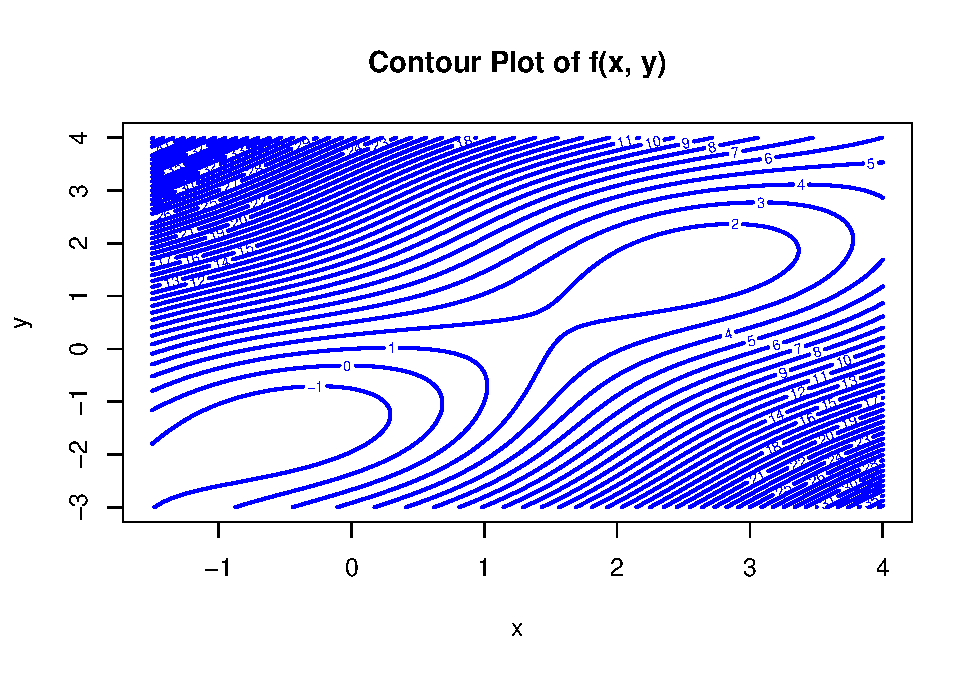
\includegraphics{732A89_lab2_files/figure-latex/unnamed-chunk-1-1.pdf}

\subsubsection{b) Derive the gradient and Hessian matrix for the
function and write R-code for
them.}\label{b-derive-the-gradient-and-hessian-matrix-for-the-function-and-write-r-code-for-them.}

\subsubsection{\texorpdfstring{c) Write your own function applying the
Newton algorithm that has the starting value \((x_0, y_0)\) as a
parameter}{c) Write your own function applying the Newton algorithm that has the starting value (x\_0, y\_0) as a parameter}}\label{c-write-your-own-function-applying-the-newton-algorithm-that-has-the-starting-value-x_0-y_0-as-a-parameter}

\subsubsection{d) Test several starting values such that you have
examples which give at least three different
results.}\label{d-test-several-starting-values-such-that-you-have-examples-which-give-at-least-three-different-results.}

\begin{verbatim}
## [1] 1.547126
## [1] 0.5471258
## Newton_algorithm gives a mimimum value at ( 1.547126 , 0.5471258 at the  6 iteration for a= 2 b= 4 
## [1] 2.594471
## [1] 1.594471
## Newton_algorithm gives a mimimum value at ( 2.594471 , 1.594471 at the  6 iteration for a= -1 b= 0 
## [1] 1.547197
## [1] 0.5471972
## Newton_algorithm gives a mimimum value at ( 1.547197 , 0.5471972 at the  6 iteration for a= -2 b= -3 
## [1] -1.594395
## [1] -2.594395
## Newton_algorithm gives a mimimum value at ( -1.594395 , -2.594395 at the  6 iteration for a= 2 b= 0
\end{verbatim}

\subsubsection{e) Investigate the candidate results which you have got.
Is one of the candidates a global minimum? Which type of solutions are
the other
candidates?}\label{e-investigate-the-candidate-results-which-you-have-got.-is-one-of-the-candidates-a-global-minimum-which-type-of-solutions-are-the-other-candidates}

The last solution gives (-1.59, -2.59) is a global minimum. (1.54,
-0.55) is the saddle point. (2.59, 1.59) is a local maximum.

\subsection{Question 2: Maximum
likelihood}\label{question-2-maximum-likelihood}

Three doses (0.1, 0.3, and 0.9 g) of a drug and placebo (0 g) are tested
in a study. Afterward, a dose-dependent event is recorded. The data of
\(n = 10\) subjects is shown in Table 1; \(x_i\) is the dose in grams;
\(y_i = 1\) if the event occurred, \(y_i = 0\) otherwise.

\begin{longtable}[]{@{}
  >{\raggedright\arraybackslash}p{(\columnwidth - 20\tabcolsep) * \real{0.1803}}
  >{\raggedright\arraybackslash}p{(\columnwidth - 20\tabcolsep) * \real{0.0820}}
  >{\raggedright\arraybackslash}p{(\columnwidth - 20\tabcolsep) * \real{0.0820}}
  >{\raggedright\arraybackslash}p{(\columnwidth - 20\tabcolsep) * \real{0.0820}}
  >{\raggedright\arraybackslash}p{(\columnwidth - 20\tabcolsep) * \real{0.0820}}
  >{\raggedright\arraybackslash}p{(\columnwidth - 20\tabcolsep) * \real{0.0820}}
  >{\raggedright\arraybackslash}p{(\columnwidth - 20\tabcolsep) * \real{0.0820}}
  >{\raggedright\arraybackslash}p{(\columnwidth - 20\tabcolsep) * \real{0.0820}}
  >{\raggedright\arraybackslash}p{(\columnwidth - 20\tabcolsep) * \real{0.0820}}
  >{\raggedright\arraybackslash}p{(\columnwidth - 20\tabcolsep) * \real{0.0820}}
  >{\raggedright\arraybackslash}p{(\columnwidth - 20\tabcolsep) * \real{0.0820}}@{}}
\toprule\noalign{}
\begin{minipage}[b]{\linewidth}\raggedright
\(x_i\) (g)
\end{minipage} & \begin{minipage}[b]{\linewidth}\raggedright
0
\end{minipage} & \begin{minipage}[b]{\linewidth}\raggedright
0
\end{minipage} & \begin{minipage}[b]{\linewidth}\raggedright
0
\end{minipage} & \begin{minipage}[b]{\linewidth}\raggedright
0.1
\end{minipage} & \begin{minipage}[b]{\linewidth}\raggedright
0.1
\end{minipage} & \begin{minipage}[b]{\linewidth}\raggedright
0.3
\end{minipage} & \begin{minipage}[b]{\linewidth}\raggedright
0.3
\end{minipage} & \begin{minipage}[b]{\linewidth}\raggedright
0.9
\end{minipage} & \begin{minipage}[b]{\linewidth}\raggedright
0.9
\end{minipage} & \begin{minipage}[b]{\linewidth}\raggedright
0.9
\end{minipage} \\
\midrule\noalign{}
\endhead
\bottomrule\noalign{}
\endlastfoot
\(y_i\) & 0 & 0 & 1 & 0 & 1 & 1 & 1 & 0 & 1 & 1 \\
\end{longtable}

Table 1: Data for Question 2

You should fit a simple logistic regression

\[ p(x) = P(Y = 1|x) = \frac{1}{1 + \exp(-\beta_0 - \beta_1 x)} \]

to the data, i.e., estimate \(\beta_0\) and \(\beta_1\). One can show
that the log likelihood is

\[ g(b) = \sum_{i=1}^{n} \left[ y_i \log\left\{(1 + \exp(-\beta_0 - \beta_1 x_i))^{-1}\right\} + (1 - y_i) \log\left\{1 - (1 + \exp(-\beta_0 - \beta_1 x_i))^{-1}\right\} \right] \]

where \(b = (\beta_0, \beta_1)^T\) and the gradient is

\[ g'(b) = \sum_{i=1}^{n} \left[ y_i - \frac{1}{1 + \exp(-\beta_0 - \beta_1 x_i)} \right] \begin{pmatrix} 1 \\ x_i \end{pmatrix} \]
```

\paragraph{\texorpdfstring{a. Write a function for an ML-estimator for
\((\beta_0, \beta_1)\) using the steepest ascent method with a
step-size-reducing line search (back-tracking).For this, you can use and
modify the code for the steepest ascent example of the lecture. The
function should count the number of function and gradient
evaluations.}{a. Write a function for an ML-estimator for (\textbackslash beta\_0, \textbackslash beta\_1) using the steepest ascent method with a step-size-reducing line search (back-tracking).For this, you can use and modify the code for the steepest ascent example of the lecture. The function should count the number of function and gradient evaluations.}}\label{a.-write-a-function-for-an-ml-estimator-for-beta_0-beta_1-using-the-steepest-ascent-method-with-a-step-size-reducing-line-search-back-tracking.for-this-you-can-use-and-modify-the-code-for-the-steepest-ascent-example-of-the-lecture.-the-function-should-count-the-number-of-function-and-gradient-evaluations.}

\begin{verbatim}
## [1] -0.009353495  1.262798921
## Steepest ascent method gives result -0.009353495 1.262799 at the  38 th iteration for -0.2 1
\end{verbatim}

\paragraph{\texorpdfstring{b. Compute the ML-estimator with the function
from a. for the data \((x_i, y_i)\) above.Use a stopping criterion such
that you can trust five digits of both parameter estimates for
\(\beta_0\) and \(\beta_1\). Use the starting value
\((\beta_0, \beta_1) = (-0.2, 1)\). The exact way to use backtracking
can be varied. Try two variants and compare the number of function and
gradient evaluations performed to
convergence.}{b. Compute the ML-estimator with the function from a. for the data (x\_i, y\_i) above.Use a stopping criterion such that you can trust five digits of both parameter estimates for \textbackslash beta\_0 and \textbackslash beta\_1. Use the starting value (\textbackslash beta\_0, \textbackslash beta\_1) = (-0.2, 1). The exact way to use backtracking can be varied. Try two variants and compare the number of function and gradient evaluations performed to convergence.}}\label{b.-compute-the-ml-estimator-with-the-function-from-a.-for-the-data-x_i-y_i-above.use-a-stopping-criterion-such-that-you-can-trust-five-digits-of-both-parameter-estimates-for-beta_0-and-beta_1.-use-the-starting-value-beta_0-beta_1--0.2-1.-the-exact-way-to-use-backtracking-can-be-varied.-try-two-variants-and-compare-the-number-of-function-and-gradient-evaluations-performed-to-convergence.}

\begin{verbatim}
## [1] -0.009353495  1.262798921
## Steepest ascent method gives result -0.009353495 1.262799 at the  38 th iteration for -0.2 1
\end{verbatim}

\begin{verbatim}
## [1] -0.009286907  1.262506751
## Steepest ascent method gives result -0.009286907 1.262507 at the  33 th iteration for 2 1
\end{verbatim}

\paragraph{\texorpdfstring{c.~Use now the function \texttt{optim} with
both the BFGS and the Nelder-Mead algorithm.Do you obtain the same
results as for b.? Is there any difference in the precision of the
result? Compare the number of function and gradient evaluations that are
given in the standard output of
\texttt{optim}.}{c.~Use now the function optim with both the BFGS and the Nelder-Mead algorithm.Do you obtain the same results as for b.? Is there any difference in the precision of the result? Compare the number of function and gradient evaluations that are given in the standard output of optim.}}\label{c.-use-now-the-function-optim-with-both-the-bfgs-and-the-nelder-mead-algorithm.do-you-obtain-the-same-results-as-for-b.-is-there-any-difference-in-the-precision-of-the-result-compare-the-number-of-function-and-gradient-evaluations-that-are-given-in-the-standard-output-of-optim.}

\begin{Shaded}
\begin{Highlighting}[]
\NormalTok{model\_BFGS}\OtherTok{\textless{}{-}} \FunctionTok{optim}\NormalTok{(}\FunctionTok{c}\NormalTok{(}\SpecialCharTok{{-}}\FloatTok{0.2}\NormalTok{,}\DecValTok{1}\NormalTok{), g, }\AttributeTok{gr=}\NormalTok{gradient, }\AttributeTok{method=}\StringTok{\textquotesingle{}BFGS\textquotesingle{}}\NormalTok{)}
\FunctionTok{print}\NormalTok{(model\_BFGS}\SpecialCharTok{$}\NormalTok{par)}
\end{Highlighting}
\end{Shaded}

\begin{verbatim}
## [1] -516.8771 -214.3395
\end{verbatim}

\begin{Shaded}
\begin{Highlighting}[]
\NormalTok{model\_nelder}\OtherTok{\textless{}{-}} \FunctionTok{optim}\NormalTok{(}\FunctionTok{c}\NormalTok{(}\SpecialCharTok{{-}}\FloatTok{0.2}\NormalTok{,}\DecValTok{1}\NormalTok{), g, }\AttributeTok{method=}\StringTok{\textquotesingle{}Nelder{-}Mead\textquotesingle{}}\NormalTok{)}
\FunctionTok{print}\NormalTok{(model\_nelder}\SpecialCharTok{$}\NormalTok{par)}
\end{Highlighting}
\end{Shaded}

\begin{verbatim}
## [1] -698.17286  -12.89984
\end{verbatim}

\paragraph{\texorpdfstring{d.~Use the function \texttt{glm} in R to
obtain an ML-solution and compare it with your results
before.}{d.~Use the function glm in R to obtain an ML-solution and compare it with your results before.}}\label{d.-use-the-function-glm-in-r-to-obtain-an-ml-solution-and-compare-it-with-your-results-before.}

\begin{Shaded}
\begin{Highlighting}[]
\NormalTok{model\_glm }\OtherTok{\textless{}{-}} \FunctionTok{glm}\NormalTok{(y }\SpecialCharTok{\textasciitilde{}}\NormalTok{ x, }\AttributeTok{family =} \FunctionTok{binomial}\NormalTok{(}\AttributeTok{link =} \StringTok{"logit"}\NormalTok{))}
\FunctionTok{summary}\NormalTok{(model\_glm)}
\end{Highlighting}
\end{Shaded}

\begin{verbatim}
## 
## Call:
## glm(formula = y ~ x, family = binomial(link = "logit"))
## 
## Coefficients:
##             Estimate Std. Error z value Pr(>|z|)
## (Intercept) -0.00936    0.87086  -0.011    0.991
## x            1.26282    1.86663   0.677    0.499
## 
## (Dispersion parameter for binomial family taken to be 1)
## 
##     Null deviance: 13.460  on 9  degrees of freedom
## Residual deviance: 12.969  on 8  degrees of freedom
## AIC: 16.969
## 
## Number of Fisher Scoring iterations: 4
\end{verbatim}

\end{document}
